\let\negmedspace\undefined
\let\negthickspace\undefined
\documentclass[journal]{IEEEtran}
\usepackage[a5paper, margin=10mm, onecolumn]{geometry}
%\usepackage{lmodern} % Ensure lmodern is loaded for pdflatex
\usepackage{tfrupee} % Include tfrupee package

\setlength{\headheight}{1cm} % Set the height of the header box
\setlength{\headsep}{0mm}     % Set the distance between the header box and the top of the text

\usepackage{gvv-book}
\usepackage{gvv}
\usepackage{cite}
\usepackage{amsmath,amssymb,amsfonts,amsthm}
\usepackage{algorithmic}
\usepackage{graphicx}
\usepackage{textcomp}
\usepackage{xcolor}
\usepackage{txfonts}
\usepackage{listings}
\usepackage{enumitem}
\usepackage{mathtools}
\usepackage{gensymb}
\usepackage{comment}
\usepackage[breaklinks=true]{hyperref}
\usepackage{tkz-euclide} 
\usepackage{listings}
% \usepackage{gvv}                                        
\def\inputGnumericTable{}                                 
\usepackage[latin1]{inputenc}                                
\usepackage{color}                                            
\usepackage{array}                                            
\usepackage{longtable}                                       
\usepackage{calc}                                             
\usepackage{multirow}                                         
\usepackage{hhline}                                           
\usepackage{ifthen}                                           
\usepackage{lscape}
\begin{document}

\bibliographystyle{IEEEtran}
\vspace{3cm}
\title{12.8.ex.9}
\author{EE24BTECH11028 - Jadhav Rajesh}
% \maketitle
% \newpage
% \bigskip
{\let\newpage\relax\maketitle}

\renewcommand{\thefigure}{\theenumi}
\renewcommand{\thetable}{\theenumi}
\setlength{\intextsep}{10pt} % Space between text and floats


\numberwithin{equation}{enumi}
\numberwithin{figure}{enumi}
\renewcommand{\thetable}{\theenumi}
 \textbf{QUESTION:} Using integration find the area of region bounded by the triangle whose verticle are $\vec(1,0),\vec(2,2)$ and $\vec(3.1)$.\\

 \textbf{SOLUTION}: \\
 \textbf{THEORETICAL SOLUTION}
 Let $A\vec(1,0),B\vec(2,2)$ and $C\vec(3.1)$ be the vertices of a triangle $ABC\brak{fig 8.18}$.\\

   Area  of $\triangle ABC = $ Area of $\triangle ABD$ $+ $  Area of trapezium $BDEC - $ Area of $\triangle AEC$ \\
   Now equation of the sides $AB,BC$ and $CA$ given by\\
 \begin{align}
     y=2\brak{x-1},y=4-x,y=\frac{1}{2}\brak{x-1},respectively.
 \end{align}\\
 Hence,   area of $\triangle ABC$
 \begin{align}
     =\int_{1}^{2}2\brak{x-1}{dx} + \int_{2}^{3}\brak{4-x}{dx} - \int_{1}^{3}\frac{x-1}{2}{dx}
 \end{align}\\
 \begin{align}
     =2\sbrak{\frac{x^{2}}{2}{-x}}_{1}^{2} +\sbrak{{4x}-\frac{x^{2}}{2}}_{2}^{3} - \frac{1}{2}\sbrak{\frac{x^{2}}{2}{-x}}_{1}^{3}
 \end{align}\\
 \begin{align}
     =2\sbrak{\brak{\frac{2^{2}}{2}{-2}}-\brak{\frac{1}{2}{-1}}} + \sbrak{\brak{4 * 3 - \frac{3^{2}}{2}} - \brak{4 * 2 - \frac{2^{2}}{2}}} - \frac{1}{2} \sbrak{\brak{\frac{3^{2}}{2}{-3}} - \brak{\frac{1}{2} -1}}
 \end{align}\\
 \begin{align}
     =\frac{3}{2}
 \end{align}\\
 \textbf{Computational Solution:}\\
Using the trapezoidal rule to get the area\\
The trapezoidal rule is as follows.\\
\begin{align}
    A &= \int_a^b f\brak{x}\,dx\approx h\brak{\frac{1}{2}f\brak{a}+f\brak{x_1}+f\brak{x_2}\dots+f\brak{x_{n-1}}+\frac{1}{2}f\brak{b}}\\
    h&=\frac{b-a}{n}\\
    A &= j_n,\quad where ,\quad j_{i+1}=j_i +h\frac{f\brak{x_{i+1}}+f\brak{x_i}}{2}\\
    j_{i+1}&= j_i+h\brak{\sqrt{x_{i+1}}+\sqrt{x_i}}\\
    x_{i+1}&=x_i +h\\
    h&=\frac{1}{30000}\\
    n&=30000
\end{align}
Using the code answer obtained is $A=1.5000sq$.units \\
\begin{figure}[h!]
   \centering
   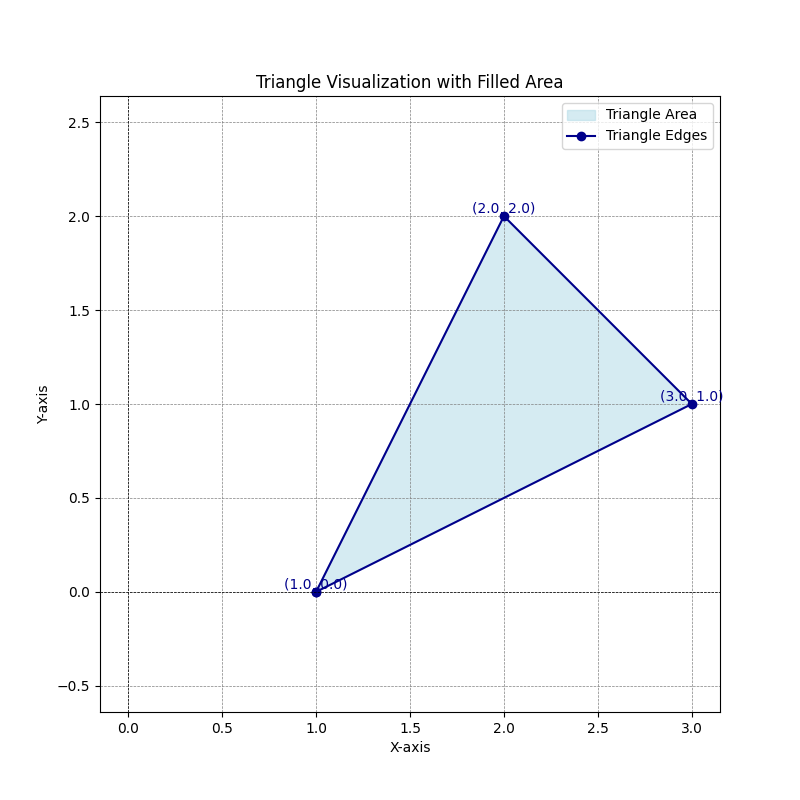
\includegraphics[width=\columnwidth]{figure/fig.png}
\end{figure}




 

 \end{document}
